\documentclass[tikz]{standalone}
\usetikzlibrary{shadings,3d,positioning,patterns}
\usepackage{ctex,amsmath,fontspec}
\definecolor{tou}{RGB}{94,125,89}
\definecolor{author}{RGB}{225,244,225}
\definecolor{title}{RGB}{255,253,127}
\definecolor{left}{RGB}{148,176,107}
\definecolor{body}{RGB}{144,192,108}
%\newcommand{\yp}[1]{{\CJKfontspec{印品赤壁赋体}#1}}
\newcommand{\fz}[1]{{\CJKfontspec{方正黑体简体}#1}}
\setmainfont{Times New Roman}
\everymath{\displaystyle}
\begin{document}
\begin{tikzpicture}
\node[minimum width=17.6cm,minimum height=25cm,inner sep=0pt,outer sep=0pt](box){};
\fill[body](box.north west)--(box.north east)--(box.south east)--(box.south west)--cycle;
\node[align=center,text=author] at (box.center)
{\zihao{-2}\fz{蒲和平} \tikz{\draw(0.25,0.25)circle(0.25);\draw(0.25,0.25)circle(0.2);} \fz{编著}\\
\zihao{-2}\fz{谢云荪} \tikz{\draw(0.25,0.25)circle(0.25);\draw(0.25,0.25)circle(0.2);} \fz{主审}};
\fill[tou](-8.8,6.5)[bend left=25]to(8.8,10.8)--(box.north east)--(box.north west)--cycle;
\fill[left color=left,right color=tou](-8.8,6.5)[bend left=24]to(8.8,10.6)
--(8.8,9.6)[bend right=23]to(-8.8,6.5);

\node[text=title,align=center,scale=6]at(0,4){\fz{大学生}\\[-0.2cm]\fz{数学竞赛教程}};
\node[opacity=0.5]at(-2,7.8){$f(x)=\lim_{n\to\infty}\sqrt[\uproot{15}n]{1+x^n+\left(\frac{x^2}2\right)^n}\,(x>0)$};
\draw[help lines,step=0.8cm,opacity=0.6](-8.8,-12.5)grid(8.8,12.5);
\node[opacity=0.5] at(5.4,7.8){\tikz{\draw[-stealth](-0.3,0)--(0,0)node[below left]{$O$}--(3.6,0)node[below=2pt]{$x$};
\draw[-stealth](0,-0.42)--(0,2)node[left]{$y$};
\draw(0,1.3)node[left]{$A$}..controls(1.4,0.6)and(2.2,2.4)..(2.8,1.7)node[right]{$B$}
--(2.8,0)node[below]{$C$};\node at(0.65,1.4){$f(x)$};}};
\node[opacity=0.5] at(-4.5,-3.5)
{
\begin{tikzpicture}[scale=1.2]
\begin{scope}[x={(-0.6cm,-0.45cm)},y={(1cm,0cm)},z={(0cm,1cm)},>=stealth]
\draw[->](0,0,0)--(2.8,0,0)node[below right,inner sep=1pt]{$x$};
\draw[->](0,0,0)--(0,2.2,0)node[below]{$y$};
\draw[->,densely dashed](0,0,0)node[below=-1pt]{$O$}--(0,0,4.7)node[left]{$z$};
\draw(0,-2.2,2)--(0,0,0)--(0,2.2,2);
\end{scope}
\draw[densely dashed](2.2,2.05)arc(0:180:2.2 and 0.4);
\draw(2.2,2.05)arc(0:-180:2.2 and 0.4);
\draw(2.2,2.05)arc(0:180:2.2 and 1.9);
\draw(-0.1,2)--(0,2)node[right]{$a$};
\node[below right,inner sep=1pt]at(0,3.9){$2a$};
\draw(-1.4,1.72)[out=73,in=200]to(0,3.95);
\draw[densely dashed](0,3.95)[out=-10,in=120]to(1.4,2.36);
\end{tikzpicture}
};
\node[opacity=0.4]at(5.5,-2){
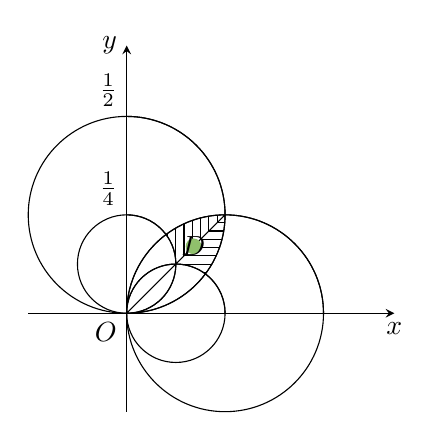
\begin{tikzpicture}[scale=10]
\begin{scope}
\clip (0,0) arc (-90:0:1/8) arc (90:180:1/8);
\fill[pattern=horizontal lines]
(0,0) arc (-90:0:1/8) --(1/16,1/16) arc (90:0:1/16);
\fill[pattern=vertical lines]
(0,0) arc (180:90:1/8) --(1/16,1/16) arc (0:90:1/16);
\end{scope}\node[below left](0,0){$O$};
\draw [-stealth](-1/8,0)--(0.34,0);\draw [-stealth](0,-1/8)--(0,0.34);
\node[below]at(0.34,0){$x$};\node[left]at(0,0.34){$y$};
\draw (0,0) arc (-90:90:1/8) (0,0) arc (-90:90:1/16)
(0,0) arc (180:0:1/8) (0,0) arc (180:0:1/16) (0,0)--(1/8,1/8);
\fill[fill=body](0.085,0.085)node[inner sep=0pt]{$D$}circle(0.01);
\draw(0,1/8)circle(1/8);\draw(0,1/16)circle(1/16);
\draw(1/8,0)circle(1/8);\draw(1/16,0)circle(1/16);
\node[above left]at(0,1/4){$\tfrac12$};\node[above left]at(0,1/8){$\tfrac14$};
\end{tikzpicture}
};
\node[opacity=0.3] at(3,-6.5){$\iiint\limits_\Omega f(x,y,z)\,\mathrm dV=\iint\limits_D\,\mathrm dx\mathrm dy\int_{z_1(x,y)}^{z_2(x,y)}f(x,y,z)\,\mathrm dz$};
\node[opacity=0.3] at(1,-8){$I_n=\int_{2n}^{2n+2}f(x-2n)\mathrm e^{-x}\,\mathrm dx\,(n=2,3,\dotsc)$};
\fill[tou](-8.8,-10.5)--(-8.8,-12.5)--(8.8,-12.5)--(8.8,-10.5)--cycle;
\node[anchor=north,align=left,text=author]at(0,-10.7){

\begin{tikzpicture}[color=author]
\draw[very thick,rounded corners](0,0)--(0,1.3)--(1.3,1.3)--(1.3,0)--cycle;
\fill(0.65,1.08)circle(0.12);
\fill(0.15,0.93)--(0.65,0.8)--(1.15,0.93)--(1.15,0.98)--(0.65,0.85)--(0.15,0.98)--cycle;
\foreach \x in{-0.12cm,-0.16cm,-0.2cm}
\fill[yshift=\x](0.15,0.93)--(0.65,0.8)--(1.15,0.93)--(1.15,0.98)--(0.65,0.85)
--(0.15,0.98)--cycle;
\foreach \x in{-0.32cm,-0.36cm,-0.4cm,-0.44cm,-0.48cm,-0.52cm,-0.56cm,-0.6cm,-0.64cm}
\fill[yshift=\x](0.15,0.93)--(0.65,0.8)--(1.15,0.93)--(1.15,0.98)--(0.65,0.85)
--(0.15,0.98)--cycle;
\end{tikzpicture}
\parbox{4cm}{\vspace{-1.2cm}
\scalebox{1.7}{\fz{电子工业出版社}}\\[-2mm]
\scalebox{0.5}[1]{PUBLISHING HOUSE OF ELECTRONICS INDUSTRY}\\[-2mm]
http//:www.phei.com.cn}
};
\end{tikzpicture}
\end{document}